\section{课本习题}
\subsection{质点运动学}

\begin{enumerate}

\item[\textbf{1-4}] 质点沿半径为$R$的圆周做匀速率运动,每间隔时间$T$转一圈.在$2T$时间间隔中,其平均速度大小和平均速率分别为(\quad)

\begin{choices}
	\item $2\pi R/T,2\pi R/T$
	\item $0,2\pi R/T$
	\item $0,0$
	\item $2\pi R/T,0$
\end{choices}


\item[\textbf{1-5}] 质点做半径为$R$的变速圆周运动时的加速度大小为(\quad)

\begin{choices}
	\item $\frac{dv}{dt}$
	\item $\frac{v^2}{R}$
	\item $\frac{dv}{dt} + \frac{v^2}{R}$
	\item $\sqrt[2]{(\frac{dv}{dt}) ^ 2 + (\frac{v^2}{R}) ^ 2}$
\end{choices}



\item[\textbf{1-12}] 质点沿半径为$R$的圆周运动,运动学方程为$\theta  = 3 + 2t^2$,则$t$时刻质点的法向加速度的大小为$a_n = \underline{\hspace{6em}}.$


\item[\textbf{1-18}] 已知质点位置矢量随时间变化的函数形式为
$\mathbf{r}=4t^2\mathbf{i}+(3+2t)\mathbf{j}\ \text{(SI单位)}.$
求:
\begin{enumerate}
	\item 质点的轨迹方程;
	\item 从 \(t=0\) 到 \(t=1\,\text{s}\) 的位移;
	\item \(t=0\) 和 \(t=1\,\text{s}\) 两时刻的速度.
\end{enumerate}


\item[\textbf{1-20}] 已知质点位置矢量随时间变化的函数形式为$\mathbf{r}=t^2\mathbf{i}+2t\mathbf{j}\ \text{(SI单位)}.$
求:
\begin{enumerate}
	\item 任一时刻的速度和加速度;
	\item 任一时刻的切向加速度和法向加速度.
\end{enumerate}

\item[\textbf{1-25}] 质点沿 \(x\) 轴运动,其加速度和位置的关系为$a=2+6x^2\ \text{(SI单位)}.$质点在 \(x=0\) 处速度为 \(10\,\text{m}\cdot\text{s}^{-1}\),试求质点在任意坐标 \(x\) 处的速度值.

\item[\textbf{1-26}] 质点沿半径为 \(1\,\text{m}\) 的圆周运动,运动学方程为
$\theta=2+3t^3\ \text{(SI单位)}.$

\begin{enumerate}
	\item 求 \(t=2\,\text{s}\) 时,质点的切向加速度和法向加速度;
	\item 当加速度的方向和半径成 \(45^\circ\) 角时,由 \(t=0\) 时刻到该时刻,其角位移是多少？
\end{enumerate}

\end{enumerate}


\newpage
\subsection{质点动力学}

\begin{enumerate}

\item[\textbf{2-5}]
质量为 \(m=0.5\,\mathrm{kg}\) 的质点,在 \(Oxy\) 平面内运动,其运动学方程为$x=5t,y=0.5t^2$从 \(t=2\,\mathrm{s}\) 到 \(t=4\,\mathrm{s}\) 这段时间内,外力对质点做的功为(\hspace{1em}).

\begin{choices}
	\item \(1.5\,\mathrm{J}\)
	\item \(3\,\mathrm{J}\)
	\item \(4.5\,\mathrm{J}\)
	\item \(-1.5\,\mathrm{J}\)
\end{choices}

\item[\textbf{2-8}]
某质点在力$\boldsymbol{F}=(4+5x)\boldsymbol{i}$的作用下沿 \(x\) 轴做直线运动,在从 \(x=0\) 移动到 \(x=10\,\mathrm{m}\) 的过程中,力 \(\boldsymbol{F}\) 所做的功为\underline{\hspace{2cm}}.


\item[\textbf{2-11}]
一质点在两恒力的共同作用下,位移为$\Delta\boldsymbol{r}=(3\boldsymbol{i}+8\boldsymbol{j})\,\mathrm{m}.$在此过程中,动能的增量为\(24\,\mathrm{J}\),已知其中一恒力$\boldsymbol{F}_1=(12\boldsymbol{i}-3\boldsymbol{j})\,\mathrm{N}$,则另一恒力所做的功为\underline{\hspace{2cm}}.

\item[\textbf{2-15}]

质量为 \(m\) 的子弹以速度 \(v_0\) 水平射入沙土中,设子弹所受阻力与速度方向相反,大小与速度成正比,比例系数为 \(k\),忽略子弹的重力,求:
\begin{enumerate}
	\item 子弹射入沙土后,速度随时间变化的函数;
	\item 子弹进入沙土的最大深度.
\end{enumerate}


\item[\textbf{2-17}]
一质量为 \(2\,\mathrm{kg}\) 的质点,在 \(Oxy\)平面上运动,受到外力$\boldsymbol{F}=4\boldsymbol{i}-24t^2\boldsymbol{j}$的作用,\(t=0\)时,它的初速度为$\boldsymbol{v}_0=(3\boldsymbol{i}+4\boldsymbol{j})\,\mathrm{m\cdot s^{-1}}$,求 \(t=1\,\mathrm{s}\) 时质点的速度及受到的法向力$F_n$.


\item[\textbf{2-25}]
一颗子弹由枪口射出时速率为 \(v_0\).当子弹在枪筒内被加速时,它所受的合力为$F=a-bt,(a,b\text{ 为常量}),$其中各个物理量均采用国际单位制.  
\begin{enumerate}
	\item 假设子弹运动到枪口处合力刚好为零,求子弹走完枪全长所需时间;
	\item 求子弹所受的冲量;
	\item 求子弹的质量.
\end{enumerate}


\item[\textbf{2-29}]
一质点所受的合力为$\boldsymbol{F}_{\text{合}}=(7\boldsymbol{i}-6\boldsymbol{j})\,\mathrm{N}.$

\begin{enumerate}
	\item 当质点从原点运动到位置$\boldsymbol{r}=(-3\boldsymbol{i}+4\boldsymbol{j}+16\boldsymbol{k})\,\mathrm{m}$时,求 \(\boldsymbol{F}_{\text{合}}\) 所做的功;
	\item 如果质点运动到 \(r\) 处需 \(0.6\,\mathrm{s}\),求合力做功的平均功率;
	\item 如果质点的质量为 \(m=1\,\mathrm{kg}\),求质点动能的变化.
\end{enumerate}


\item[\textbf{2-31}]
一人用质量为 \(1\,\mathrm{kg}\) 的水桶从深为 \(10\,\mathrm{m}\) 的井中提水,水桶刚离开水面时桶中装有 \(10\,\mathrm{kg}\) 的水.由于木桶漏水,每升高 \(1\,\mathrm{m}\) 要匀漏去\(0.2\,\mathrm{kg}\)的水.若人把木桶匀速地从水面提到井口,在此过程中需做多少功？


\item[\textbf{2-38}]
质量为 \(m'\) 的大木块具有半径为 \(R\) 的四分之一弧形槽,如图~\ref{fig:2-38}~所示.质量为 \(m\) 的小球从曲面的顶端滑下,大木块放在光滑水平面上,二者都做无摩擦的运动,且都从静止开始,求小球脱离大木块时的速度.

\begin{figure}[H]
	\centering
	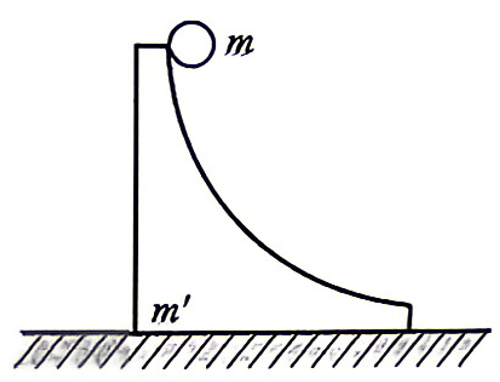
\includegraphics[width=0.3\linewidth]{figures/2-38}
	\caption{习题2-38图}
	\label{fig:2-38}
\end{figure}

\end{enumerate}

\newpage
\subsection{刚体的力学基础}
\begin{enumerate}

\item[\textbf{3-10}]
固定在一起的两个同轴均匀圆柱体可绕其光滑的水平对称轴 \(OO'\) 转动.设大小圆柱体的半径分别为 \(R\) 和 \(r\),质量分别为 \(m'\) 和 \(m\).绕在两柱体上的细绳分别与物体 \(m_1\) 和 \(m_2\) 相连,\(m_1\) 和 \(m_2\) 则挂在圆柱体的两侧,如图~\ref{fig:3-10}~所示.设 \(R=0.20\,\mathrm{m}\),\(r=0.10\,\mathrm{m}\),\(m=4\,\mathrm{kg}\),\(m'=10\,\mathrm{kg}\),\(m_1=m_2=2\,\mathrm{kg}\),且开始时 \(m_1\) 和 \(m_2\) 离地高度均为 \(h=2\,\mathrm{m}\).


\begin{figure}[H]
	\centering
	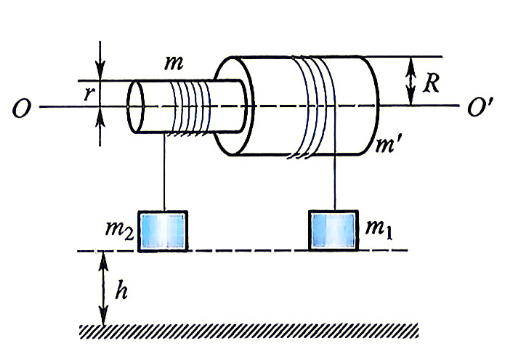
\includegraphics[width=0.2\linewidth]{figures/3-10}
	\caption{习题3-10图}
	\label{fig:3-10}
\end{figure}


\begin{enumerate}
	\item 求柱体转动时的角加速度;
	\item 求两侧细绳的张力;
	\item $m_1$ 和 $m_2$ 哪个先落地？它落地前瞬间的速率为多少？
\end{enumerate}

\item[\textbf{3-11}]
计算如图~\ref{fig:3-11}~所示系统中物体的加速度大小.设滑轮为质量均匀分布的圆柱体,半径为 \(r=0.1\,\mathrm{m}\),轻绳不可伸长,且与滑轮之间无相对滑动,滑轮轴上摩擦不计,且忽略桌面与物体 \(m_1\) 间的摩擦,已知 \(m_1=50\,\mathrm{kg}\),\(m_2=200\,\mathrm{kg}\),滑轮质量 \(m'=15\,\mathrm{kg}\).

\begin{figure}[H]
	\centering
	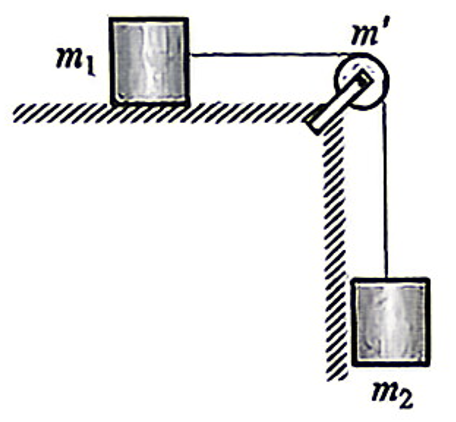
\includegraphics[width=0.3\linewidth]{figures/3-11}
	\caption{习题3-11图}
	\label{fig:3-11}
\end{figure}


\item[\textbf{3-12}]
如图~\ref{fig:3-12}~所示,一匀质细杆质量为 \(m\),长为 \(l\),可绕过一端 \(O\) 的水平光滑固定轴转动,杆从水平位置由静止开始摆下.求:
\begin{figure}[H]
	\centering
	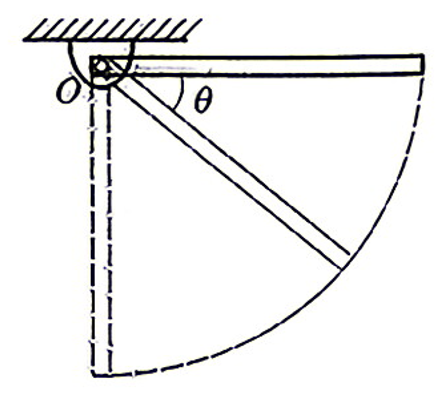
\includegraphics[width=0.2\linewidth]{figures/3-12}
	\caption{习题3-12图}
	\label{fig:3-12}
\end{figure}

\begin{enumerate}
	\item 初始时刻的角加速度;
	\item 杆转过 \(\theta\) 角时的角加速度和角速度.
\end{enumerate}


\item[\textbf{3-13}]
如图~\ref{fig:3-13}~所示,一长为 \(1\,\mathrm{m}\) 的均匀直棒可绕其一端与棒垂直的水平光滑固定轴转动,抬起另一端使棒向上与水平面成 \(60^\circ\) 角,然后无初速度地将棒释放,求:
\begin{enumerate}
	\item 放手时棒的角加速度;
	\item 棒转到竖直位置时的角速度.
\end{enumerate}

\begin{figure}[H]
	\centering
	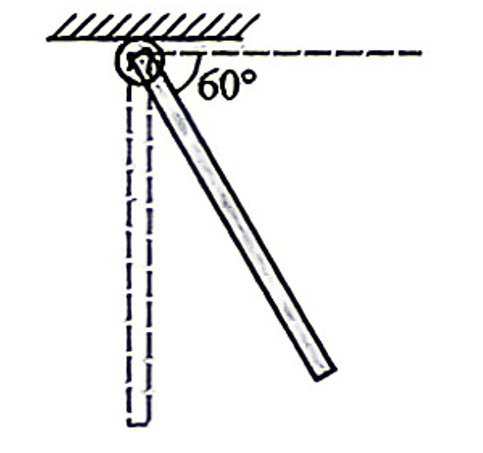
\includegraphics[width=0.3\linewidth]{figures/3-13}
	\caption{习题3-13图}
	\label{fig:3-13}
\end{figure}


\item[\textbf{3-14}]
如图~\ref{fig:3-14}~所示,长为 \(L\)、质量为 \(m\) 的均匀细杆静止在水平桌面上,可绕通过左端 \(O\) 点的竖直光滑轴转动.一质量为 \(m_0=m/3\) 的小球以速度 \(v_0\) 垂直击杆于 \(P\) 点,并以速度 \(v=v_0/3\) 弹回.设 \(OP=(3/4)L\),杆与水平面间的摩擦系数为 \(\mu\).求:
\begin{enumerate}
	\item 开始转动时的角速度;
	\item 杆所受摩擦力矩的大小;
	\item 杆从开始转动到静止所转过的角度和经历的时间.
\end{enumerate}

\begin{figure}[H]
	\centering
	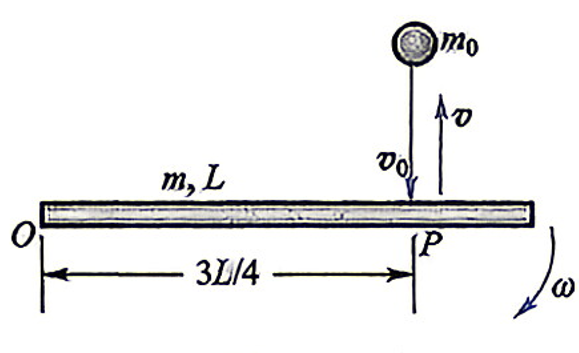
\includegraphics[width=0.3\linewidth]{figures/3-14}
	\caption{习题3-14图}
	\label{fig:3-14}
\end{figure}

\item[\textbf{3-16}]
有一质量为 \(m_1\)、长为 \(l\) 的均匀的细棒 \(OA\),可绕一端的水平固定轴 \(O\) 自由转动,初始时静止悬挂.一水平运动的质量为 \(m_2\) 的小球,从侧面垂直于棒和轴与棒的另一端 \(A\) 相碰撞,设碰撞时间极短.已知小球在碰撞前后的速度分别为 \(v_1\)、\(v_2\),方向如图~\ref{fig:3-16}~所示.求:
\begin{enumerate}
	\item 碰撞后瞬间细棒的角速度;
	\item 细棒能够摆动的最大摆角 \(\theta_m\).
\end{enumerate}

\begin{figure}[H]
	\centering
	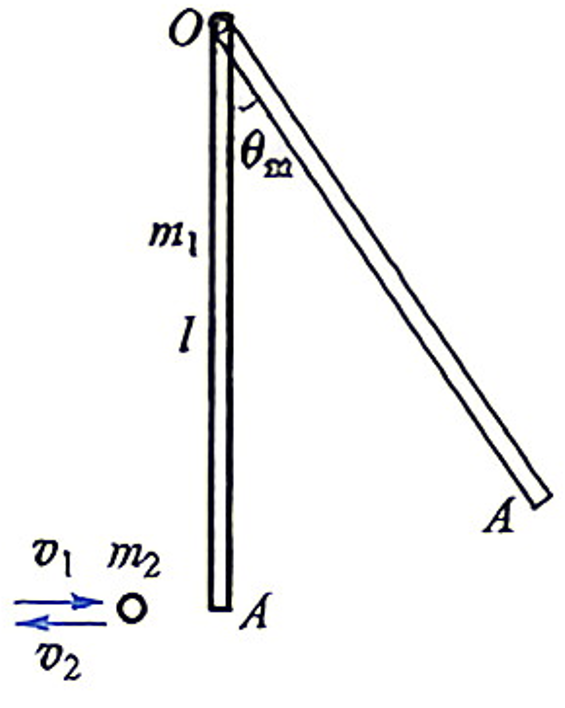
\includegraphics[width=0.2\linewidth]{figures/3-16}
	\caption{习题3-16图}
	\label{fig:3-16}
\end{figure}


\item[\textbf{3-17}]
如图~\ref{fig:3-17}~所示,一长为 \(l\)、质量为 \(m_1\) 的均质细杆,可绕通过其一端的水平轴 \(O\) 在竖直平面内自由转动,杆从水平位置由静止释放后,与 \(O\) 点正下方静止在光滑水平面上的物体 \(m_2\) 发生碰撞,\(m_2=m_1/3\).求:
\begin{enumerate}
	\item 杆在转动过程中角加速度 \(\alpha\) 的表达式;
	\item 杆转到竖直位置时的角动量和动能;
	\item 若碰撞是完全弹性的,碰撞后 \(m_2\) 的速度;
	\item 弹簧被压缩的最大长度.
\end{enumerate}

\begin{figure}[H]
	\centering
	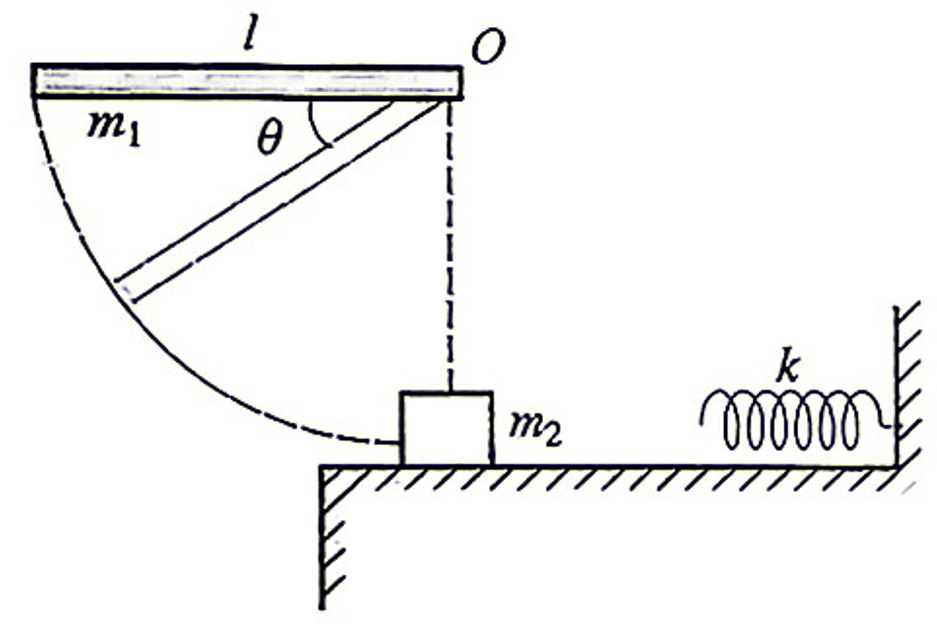
\includegraphics[width=0.3\linewidth]{figures/3-17}
	\caption{习题3-17图}
	\label{fig:3-17}
\end{figure}

\end{enumerate}


\newpage
\subsection{机械振动与机械波}

\begin{enumerate}

\item[\textbf{4-7}]
一平面简谐波在弹性介质中传播,在某一瞬时,介质中某质元正处于平衡位置,此时它的(\quad)
\begin{choices}
	\item 动能为零,势能最大.
	\item 动能为零,势能为零.
	\item 动能最大,势能最大.
	\item 动能最大,势能为零.
\end{choices}

\item[\textbf{4-11}]
两个同方向同频率的简谐振动,其合振动的振幅为 $20\,\mathrm{cm}$,与第一个简谐振动的相位差 $\varphi-\varphi_1$ 为 $\pi/6$.若第一个简谐振动的振幅为 $10\sqrt{3}\,\mathrm{cm}\approx17.3\,\mathrm{cm}$,则第二个简谐振动的振幅为\underline{\hspace{2.5cm}}$\mathrm{cm}$,第一、第二两个简谐振动的相位差 $\varphi_1-\varphi_2$ 为\underline{\hspace{2.5cm}}.

\item[\textbf{4-15}]
原长为 $0.5\,\mathrm{m}$ 的弹簧,上端固定,下端挂一个质量为 $0.1\,\mathrm{kg}$ 的物体;当物体静止时,弹簧长为 $0.6\,\mathrm{m}$.现将物体上推,使弹簧缩回到原长,然后放手,以放手时开始计时,取竖直向下为正方向,写出振动表达式(取 $g=9.8\,\mathrm{m\cdot s^{-2}}$).

\item[\textbf{4-17}]
简谐振动的振动曲线如图~\ref{fig:4-17}~所示,求振动方程.

\begin{figure}[H]
	\centering
	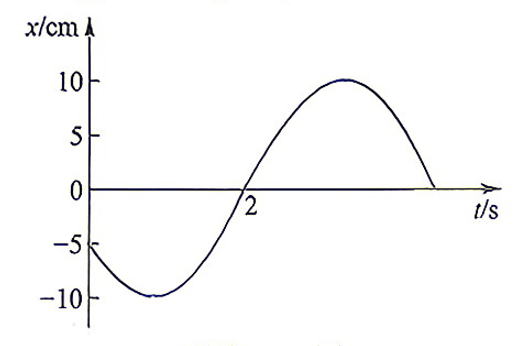
\includegraphics[width=0.3\linewidth]{figures/4-17}
	\caption{习题4-17图}
	\label{fig:4-17}
\end{figure}


\item[\textbf{4-18}]
一个质点沿 $x$ 轴做简谐振动,振幅为 $12\,\mathrm{cm}$,周期为 $2\,\mathrm{s}$.当 $t=0$ 时,位移为 $6\,\mathrm{cm}$,且向 $x$ 轴正方向运动.
\begin{enumerate}
	\item 求振动表达式;
	\item 求 $t=0.5\,\mathrm{s}$ 时,质点的位置、速度和加速度;
	\item 如果在某时刻质点位于 $x=-6\,\mathrm{cm}$,且向 $x$ 轴负方向运动,求从该位置回到平衡位置所需要的最短时间.
\end{enumerate}

\item[\textbf{4-19}]
弹簧振子沿 $x$ 轴做简谐振动.已知振动体最大位移为 $x_m=0.4\,\mathrm{m}$时最大回复力大小为 $F_{m}=0.8\,\mathrm{N}$,最大速度为 $v_m=0.8\pi\,\mathrm{m\cdot s^{-1}}$,又知 $t=0$ 的位移为 $+0.2\,\mathrm{m}$,且初速度与所选 $x$ 轴方向相反.求:
\begin{enumerate}
	\item 振动的能量;
	\item 该振动的表达式.
\end{enumerate}

\item[\textbf{4-21}]
两个同方向同频率的简谐振动曲线如图~\ref{fig:4-21}~所示.
\begin{enumerate}
	\item 求合振动的振幅;
	\item 求合振动的表达式.
\end{enumerate}

\begin{figure}[H]
	\centering
	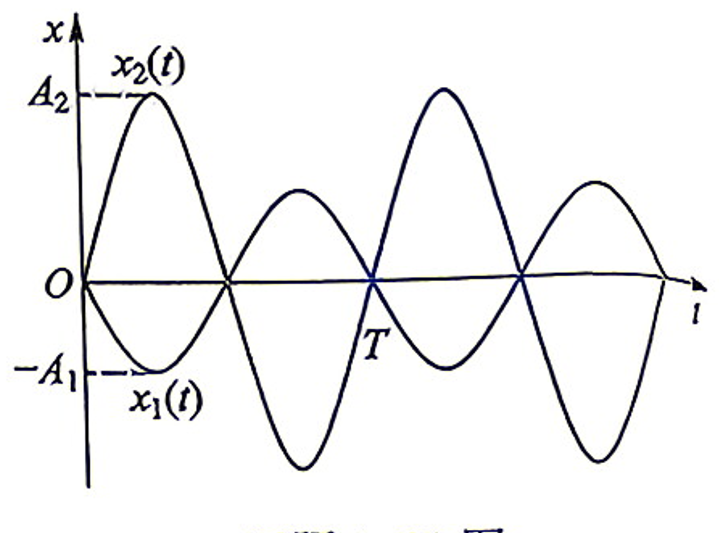
\includegraphics[width=0.4\linewidth]{figures/4-21}
	\caption{习题4-21图}
	\label{fig:4-21}
\end{figure}


\item[\textbf{4-22}]
已知一平面简谐波的波函数为$y=0.25\cos(125t-0.37x)\quad (\mathrm{SI}\ \text{单位})$分别求:
\begin{enumerate}
	\item $x_1=10\,\mathrm{m}$ 和 $x_2=25\,\mathrm{m}$ 两点处质元的振动方程;
	\item $x_1$ 和 $x_2$ 两质点间的振动相位差;
	\item $t=4\,\mathrm{s}$ 时 $x_1$ 点的振动位移.
\end{enumerate}

\item[\textbf{4-24}]
图~\ref{fig:4-24}~示为一平面简谐波在 $t=0$ 时刻的波形图,求:
\begin{enumerate}
	\item 该波的波函数;
	\item $P$ 处质元的振动方程.
\end{enumerate}

\begin{figure}[H]
	\centering
	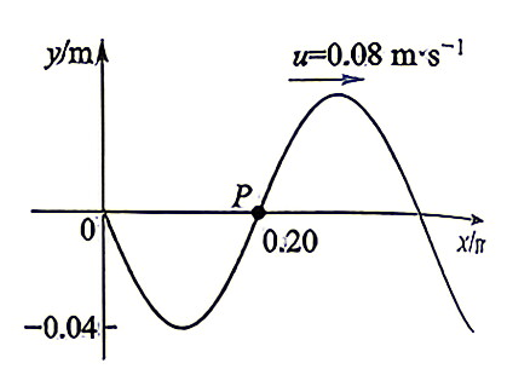
\includegraphics[width=0.3\linewidth]{figures/4-24}
	\caption{习题4-24图}
	\label{fig:4-24}
\end{figure}


\item[\textbf{4-25}]
已知一沿 $x$ 正方向传播的平面余弦波,$t=\dfrac{1}{3}\,\mathrm{s}$ 时刻的波形如图~\ref{fig:4-25}~所示,且周期 $T$ 为 $2\,\mathrm{s}$.

\begin{figure}[H]
	\centering
	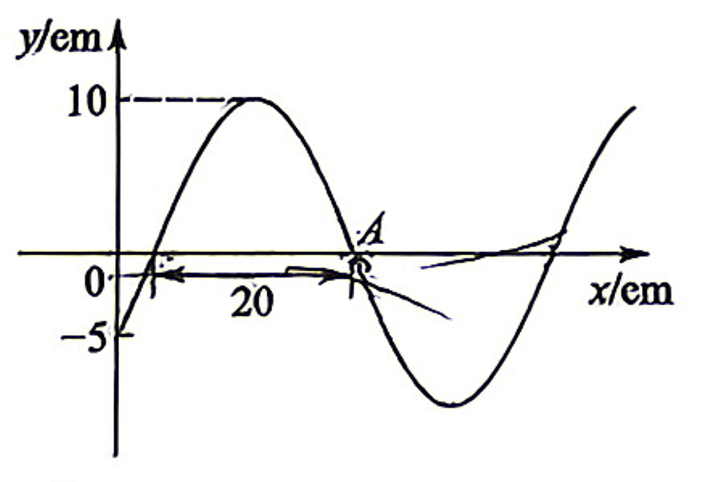
\includegraphics[width=0.4\linewidth]{figures/4-25}
	\caption{习题4-25图}
	\label{fig:4-25}
\end{figure}


\begin{enumerate}
	\item 写出 $O$ 点的振动表达式;
	\item 写出该波的波函数;
	\item 写出 $A$ 点的振动表达式;
	\item 写出 $A$ 点离 $O$ 点的距离.
\end{enumerate}

\item[\textbf{4-26}]
一平面简谐波以波速度 $u=0.8\,\mathrm{m\cdot s^{-1}}$ 沿 $x$ 轴负方向传播,已知原点的振动曲线如图~\ref{fig:4-26}~所示.试写出:
\begin{enumerate}
	\item 原点的振动表达式;
	\item 波函数;
	\item 同一时刻相距 $1\,\mathrm{m}$ 的两点之间的相位差.
\end{enumerate}

\begin{figure}[H]
	\centering
	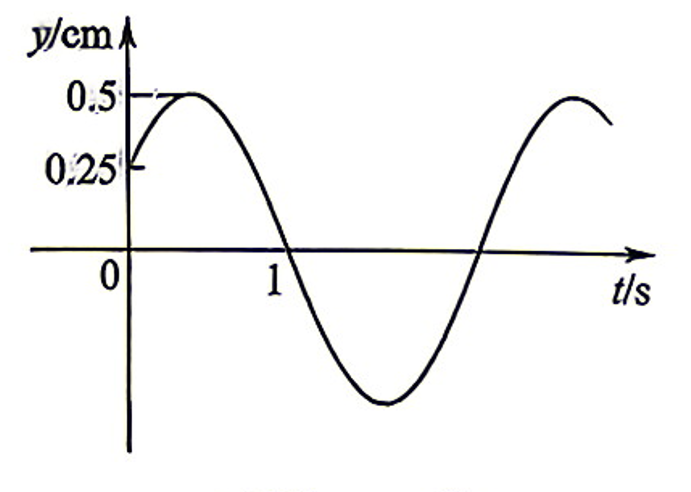
\includegraphics[width=0.3\linewidth]{figures/4-26}
	\caption{习题4-26图}
	\label{fig:4-26}
\end{figure}


\item[\textbf{4-30}]
设 $S_1$ 与 $S_2$ 为两个相干波源,相距 $\dfrac{1}{4}$ 波长,$S_1$ 比 $S_2$ 的相位超前 $\dfrac{\pi}{2}$.若两波在 $S_1$、$S_2$ 连线方向上的强度相同且不随距离变化,问 $S_1$、$S_2$ 连线上在 $S_1$ 外侧各点合成波的强度如何？在 $S_2$ 外侧各点的强度又如何？	
	
\end{enumerate}


\newpage
\subsection{真空中的静电场}

\begin{enumerate}

\item[\textbf{7-9}] 一个细玻璃棒被弯成半径为 $R$ 的半圆形,沿其上半部分均匀分布有电荷 $+Q$,沿其下半部分均匀分布有电荷 $-Q$,如习题图~\ref{fig:7-9}~所示.试求圆心 $O$ 处的电场强度.


\begin{figure}[H]
	\centering
	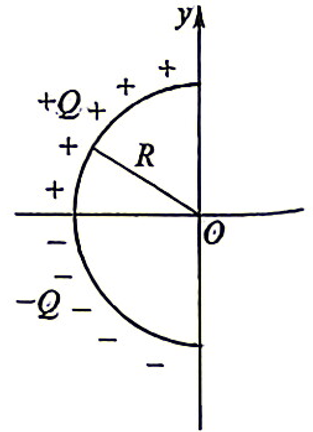
\includegraphics[width=0.2\linewidth]{figures/7-9}
	\caption{习题7-9图}
	\label{fig:7-9}
\end{figure}


\item[\textbf{7-11}] 如图~\ref{fig:7-11}~所示,两个无限大的平行平面都均匀带电,电荷的面密度分别为 $\sigma_1$ 和 $\sigma_2$,试求空间各处场强.


\begin{figure}[H]
	\centering
	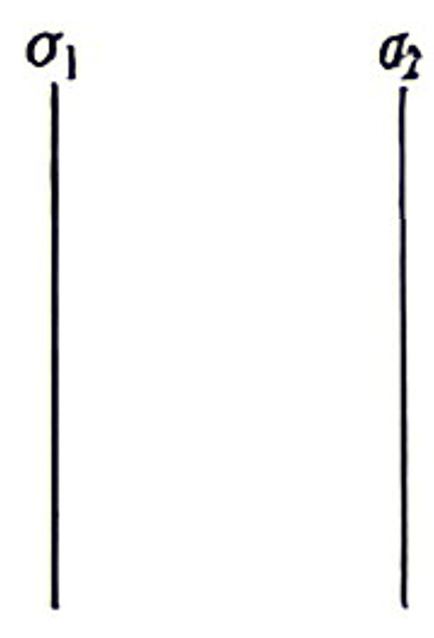
\includegraphics[width=0.2\linewidth]{figures/7-11}
	\caption{习题7-11图}
	\label{fig:7-11}
\end{figure}



\item[\textbf{7-13}] 如图~\ref{fig:7-13}~所示,在点电荷 $q$ 的电场中,选取以 $q$ 为中心、$R$ 为半径的球面上一点 $P$ 作为电势零点,求与点电荷 $q$ 距离为 $r$ 的 $P'$ 点的电势.



\begin{figure}[H]
	\centering
	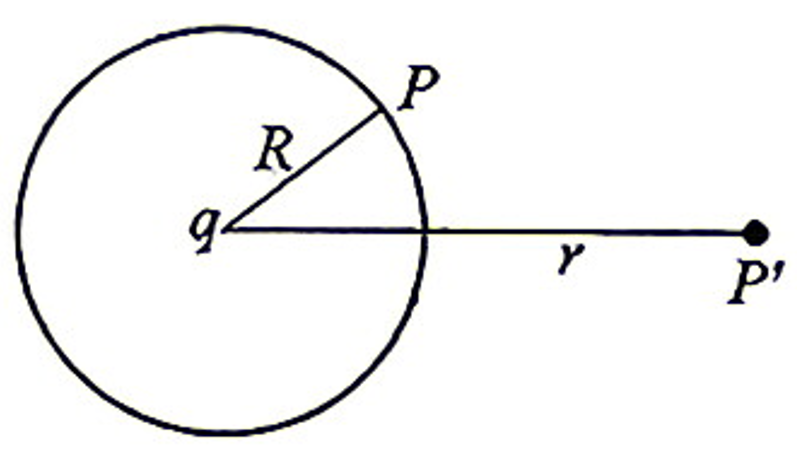
\includegraphics[width=0.3\linewidth]{figures/7-13}
	\caption{习题7-13图}
	\label{fig:7-13}
\end{figure}


\item[\textbf{7-14}] 如图~\ref{fig:7-14}~所示,边长为 $a$ 的等边三角形的三个顶点上,分别放置着三个正的点电荷 $q$、$2q$、$3q$.若将另一正点电荷 $Q$ 从无穷远处移到三角形的中心 $O$ 处,外力所做的功多大？


\begin{figure}[H]
	\centering
	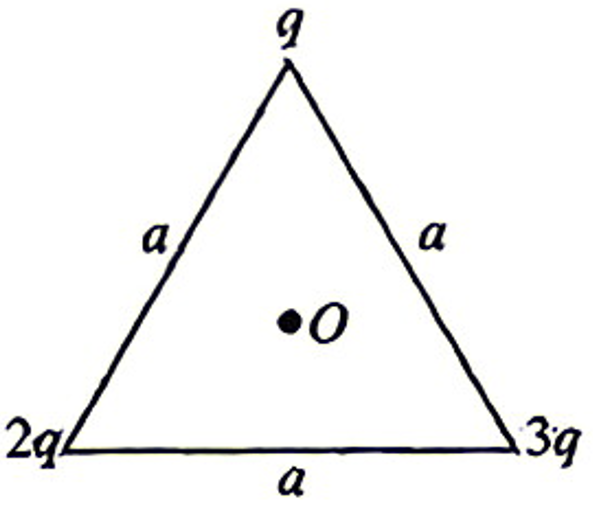
\includegraphics[width=0.3\linewidth]{figures/7-14}
	\caption{习题7-14图}
	\label{fig:7-14}
\end{figure}


\item[\textbf{7-15}] 如图~\ref{fig:7-15}~所示,试验电荷 $q$ 在点电荷 $+Q$ 产生的电场中,沿半径为 $R$ 的整个圆弧的 $3/4$ 圆弧轨道,由 $a$ 点移到 $d$ 点的过程中电场力做的功为多少？从 $d$ 点移到无限远处的过程中,电场力做的功为多少？


\begin{figure}[H]
	\centering
	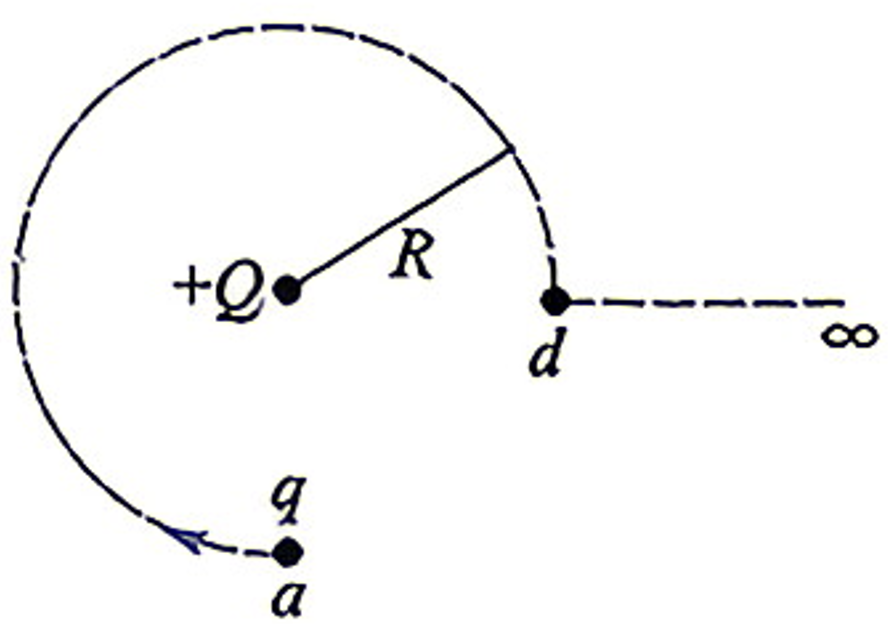
\includegraphics[width=0.3\linewidth]{figures/7-15}
	\caption{习题7-15图}
	\label{fig:7-15}
\end{figure}


\item[\textbf{7-17}] 电荷 $q$ 均匀分布在长为 $2l$ 的细杆上,求在杆外延长线上与杆端距离为 $a$ 的 $P$ 点的电势(设无限远处为电势零点).


\item[\textbf{L7-2}]
设电荷$q$均匀分布在半径为$a$的圆环上,计算在环的轴线上与环心相距$x$的$P$点的场强.

\begin{figure}[H]
	\centering
	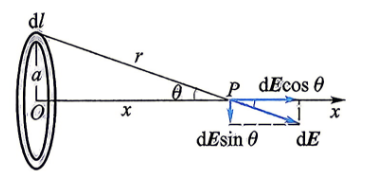
\includegraphics[width=0.3\linewidth]{figures/L7-2}
	\caption{例题L7-2辅助图}
	\label{fig:L7-2}
\end{figure}

\item[\textbf{L7-5}]
均匀带电球面的场强.设有一均匀带电球面,半径为$R$,电荷为$+q$,求球面内外任一点场强.


\begin{figure}[H]
	\centering
	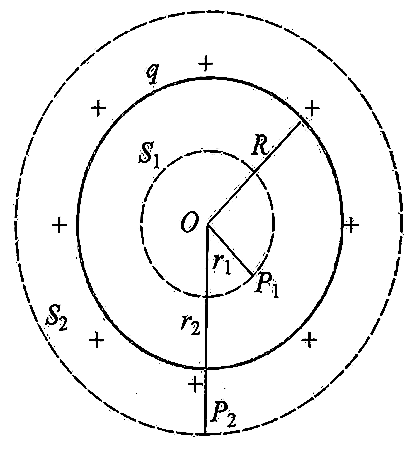
\includegraphics[width=0.3\linewidth]{figures/L7-5}
	\caption{例题L7-5辅助图}
	\label{fig:L7-5}
\end{figure}


\item[\textbf{L7-7}]
无限长均匀带电圆柱面,半径为 $R$,电荷面密度 $\sigma>0$,求柱面内外任一点场强.

\begin{figure}[H]
	\centering
	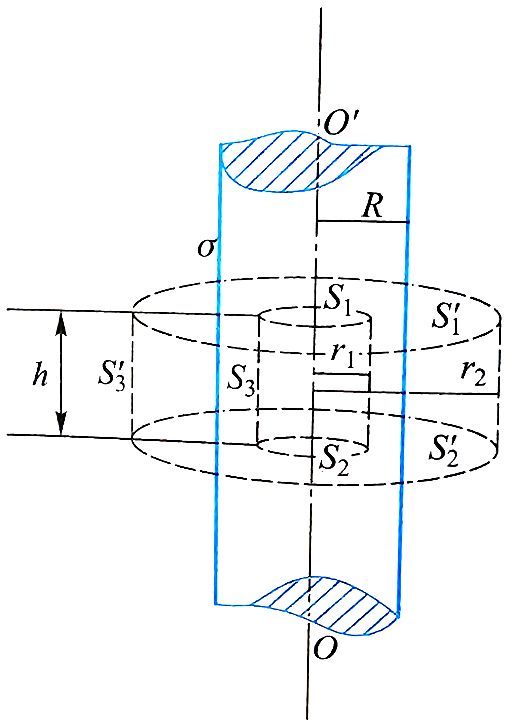
\includegraphics[width=0.3\linewidth]{figures/L7-7}
	\caption{例题L7-7辅助图}
	\label{fig:L7-7}
\end{figure}

\item[\textbf{L7-9}]
有两个厚度不计的平行无限大均匀带电平板 $A$、$B$,电荷面密度分别为
\begin{enumerate}
	\item $+\sigma,\,+\sigma$;
	\item $+\sigma,\,-\sigma$.
\end{enumerate}

请分别求板内、外的场强.

\begin{figure}[H]
	\centering
	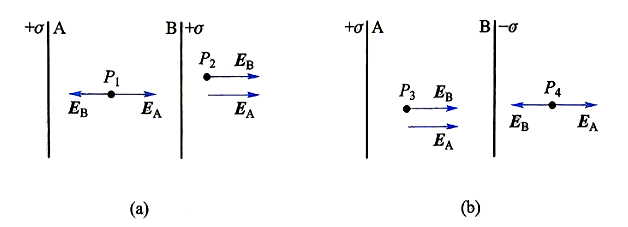
\includegraphics[width=0.5\linewidth]{figures/L7-9}
	\caption{例题L7-9辅助图}
	\label{fig:L7-9}
\end{figure}

\item[\textbf{L7-11}]
一个均匀带电球面,半径为 $R$,电荷为 $q$,求球面内、外任一点电势.

\begin{figure}[H]
	\centering
	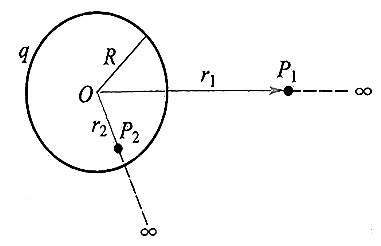
\includegraphics[width=0.3\linewidth]{figures/L7-11}
	\caption{例题L7-11辅助图}
	\label{fig:L7-11}
\end{figure}


\item[\textbf{L7-12}]
如图~\ref{fig:L7-12}~所示,有两个均匀带电的同心球面,半径分别为 $R_1$、$R_2$,电荷分别为 $+q$、$-q$,求两球面的电势差 $U$.

\begin{figure}[H]
	\centering
	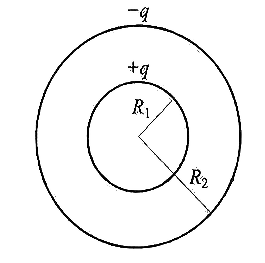
\includegraphics[width=0.3\linewidth]{figures/L7-12}
	\caption{例题L7-12图}
	\label{fig:L7-12}
\end{figure}

\end{enumerate}


\newpage
\subsection{导体和电介质}

\begin{enumerate}

\item[\textbf{8-5}] 电荷量$Q$均匀分布在半径为$R$的球体内,则球内,球外的静电能之比为$\underline{\hspace{2cm}}$.

\item[\textbf{L8-1}]
半径为$a$的两平行长直导线相距为$d$($d$远远大于$a$),二者电荷线密度为$+\lambda$、$-\lambda$,试求：

\begin{figure}[H]
	\centering
	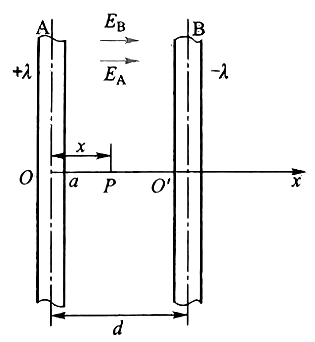
\includegraphics[width=0.3\linewidth]{figures/L8-1}
	\caption{例题L8-1辅助图}
	\label{fig:L8-1}
\end{figure}


\begin{enumerate}
	\item 两导线间电势差;
	\item 此导线组单位长度的电容.
\end{enumerate}



\item[\textbf{L8-2}]
有一个带电为 $+q$、半径为 $R_1$ 的导体球,与内外半径分别为 $R_3, R_4$、带电荷为 $-q$ 的导体球壳同心,两者之间有两层均匀电介质,内层和外层电介质的电容率分别为 $\varepsilon_1, \varepsilon_2$,且两电介质分界面也是与导体球同心的半径为 $R_2$ 的球面.试求：

\begin{figure}[H]
	\centering
	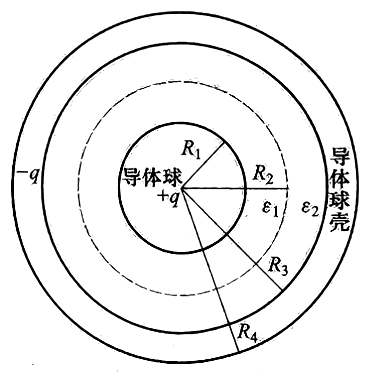
\includegraphics[width=0.3\linewidth]{figures/L8-2}
	\caption{例题L8-2辅助图}
	\label{fig:L8-2}
\end{figure}

\begin{enumerate}
	\item 电位移分布;
	\item 场强分布;
	\item 导体球与导体球壳间的电势差;
	\item 导体球壳构成电容器的电容.

\end{enumerate}

\end{enumerate}

\newpage

\subsection{恒定磁场}

\begin{enumerate}
	\item [\textbf{9-10}]
	无限长细导线弯成如图~\ref{fig:9-10}~所示acd的形状，其中c部分是在$Oxy$平面内半径为$\mathbf{R}$的半圆，求通以电流$\textbf{\textit{I}}$时$\mathbf{O}$点的磁感应强度.
	
	\begin{figure}[H]
		\centering
		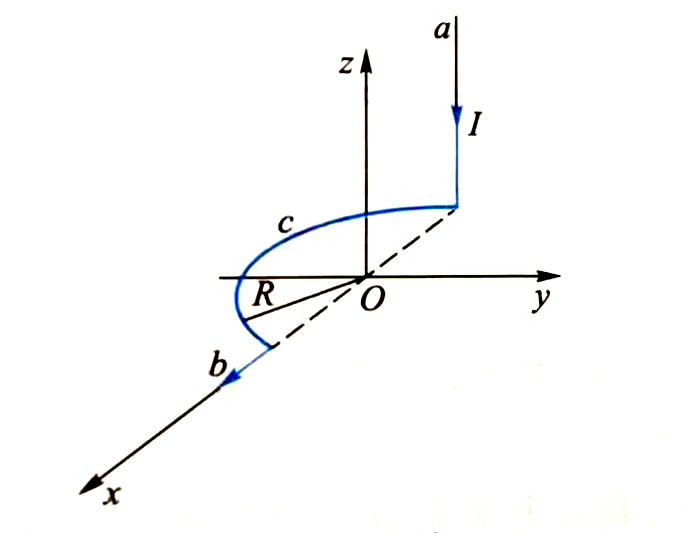
\includegraphics[width=0.4\linewidth]{figures/9-10}
		\caption{习题9-10图}
		\label{fig:9-10}
	\end{figure}
	
	\item [\textbf{9-12}]
	如图~\ref{fig:9-12}~所示，AB、CD为长直导线，$\overset{\LARGE{\frown}}{BC}$为圆心在$O$点的一段圆弧形导线，其半径为$\mathbf{R}$.若通以电流$\textit{I}$,求$O$点的磁感应强度.
	
	\begin{figure}[H]
		\centering
		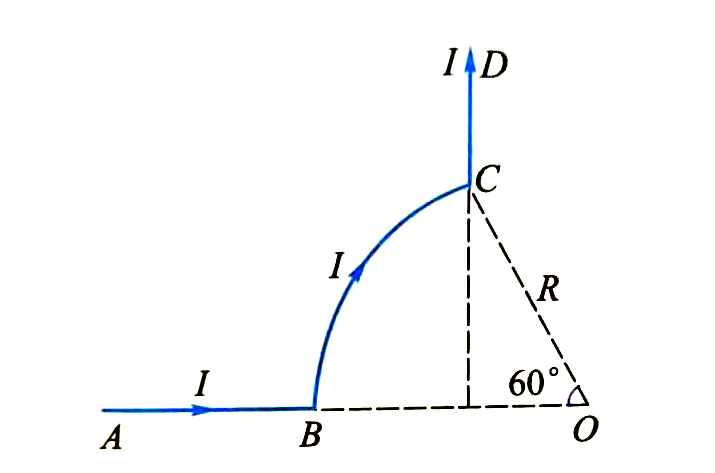
\includegraphics[width=0.4\linewidth]{figures/9-12}
		\caption{习题9-12图}
		\label{fig:9-12}
	\end{figure}
	
	\item [\textbf{9-15}]
	两平行长直导线相距$\textit{d}=40\,\text{cm}$,每根导线载有电流$\boldsymbol{I}_1=\boldsymbol{I}_2=20A$,如图~\ref{fig:9-15}~所示.求
	\begin{enumerate}
		\item [(1)] 两导线所在平面内与该两导线等距的一点A处的磁感应强度：
		\item [(2)] 通过图中方框面积的磁通量.($r_1=r_3=10cm,l=25cm.$)
	\end{enumerate}
	
	\begin{figure}[H]
		\centering
		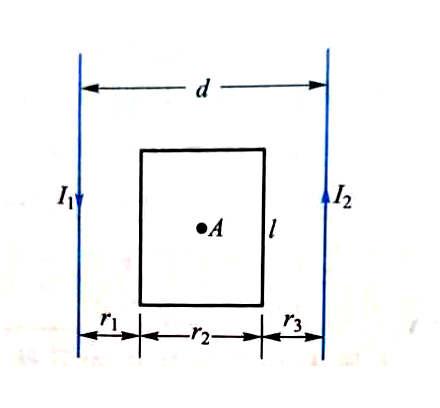
\includegraphics[width=0.3\linewidth]{figures/9-15}
		\caption{习题9-15图}
		\label{fig:9-15}
	\end{figure}
	
	\item [\textbf{9-16}]
	长直电缆由半径为$\mathbf{R_1}$的导体圆柱与同轴的内外半径分别为$\mathbf{R_2}$、$\mathbf{R_2}$的导体圆筒构成，电流沿轴线方向由一导体流入，从另一导体流出，设电流$\textit{I}$均匀地分布在横截面上.求距轴线为r处的磁感应强度大小$(0<r<\infty)$.
	
	\item [\textbf{9-19}]
	半径为$\textbf{R}$的半圆形闭合线圈，载有电流$\textit{I}$，放在均匀磁场中，磁场方向与线圈平面平行，如图~\ref{fig:9-19}~所示.
	\begin{enumerate}
		\item [(1)] 求线圈所受力矩的大小和方向(以直径为转轴);
		\item [(2)] 若线圈受上述磁场作用转到线圈平面与磁场垂直的位置，则力矩做的功为多少？
	\end{enumerate}
	
	\begin{figure}[H]
		\centering
		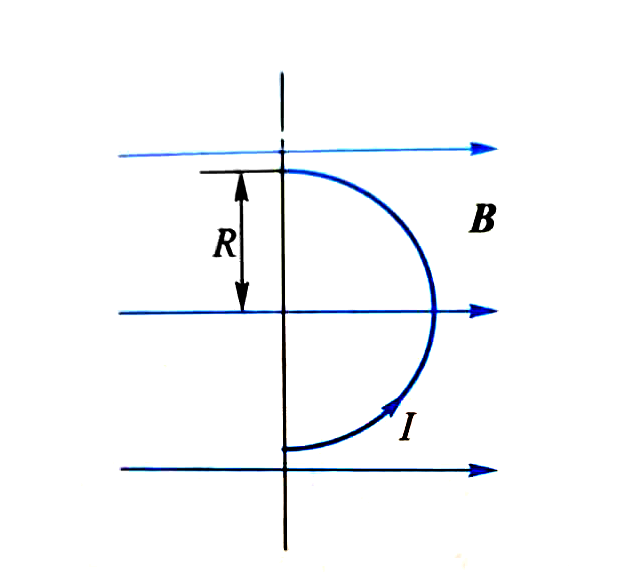
\includegraphics[width=0.3\linewidth]{figures/9-19}
		\caption{习题9-19图}
		\label{fig:9-19}
	\end{figure}
	
	\item [\textbf{9-20}]
	如图~\ref{fig:9-20}~所示，在长直导线AB内通以电流$\boldsymbol{I_1}=20A$，在矩形线圈CDEF中通以电流$\boldsymbol{I_2}=10A$，AB与线圈共面，且CD、EF都与AB平行.已知$a=9.0cm,b=20.0cm,d=1.0cm$，求:
	\begin{enumerate}
		\item [(1)] 导线AB的磁场对矩形线圈每边所作用的力;
		\item [(2)] 矩形线圈所受合力和合力矩.
	\end{enumerate}
	
	\begin{figure}[H]
		\centering
		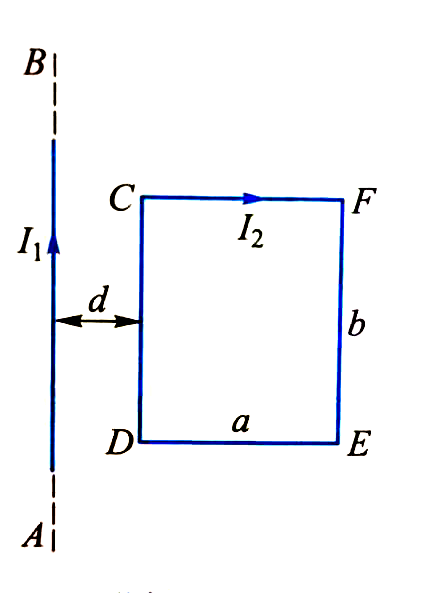
\includegraphics[width=0.25\linewidth]{figures/9-20}
		\caption{习题9-20图}
		\label{fig:9-20}
	\end{figure}
	
	\item[\textbf{L9-2}] 如图~\ref{fig:L9-2}~所示，一无限长载流直导线 $AB$，载有大小为 $I_1$ 的电流，在它的一侧有一长为 $l$ 的有限长载流直导线 $CD$，其电流为 $I_2$，$AB$ 与 $CD$ 共面，且 $CD \perp AB$，$C$ 端距 $AB$ 为 $a$.求 $CD$ 受到的安培力.
	
	\begin{figure}[H]
		\centering
		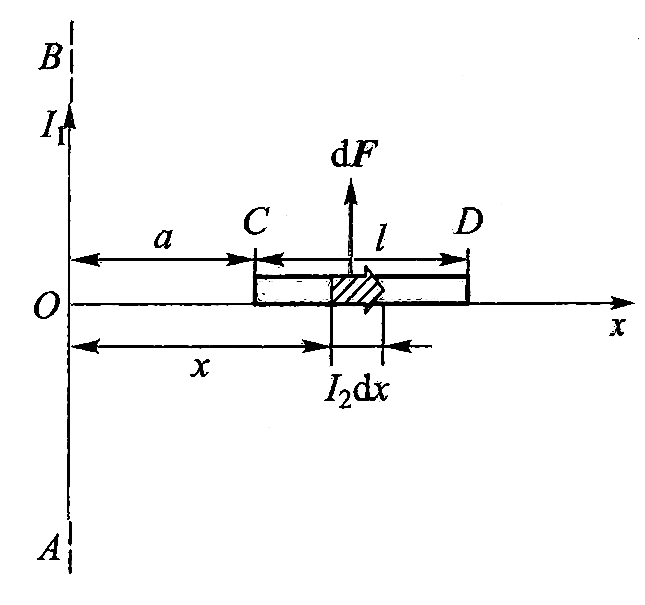
\includegraphics[width=0.4\linewidth]{figures/L9-2}
		\caption{例题9-2图}
		\label{fig:L9-2}
	\end{figure}
	
	
\end{enumerate}

\newpage
\subsection{变化的电磁场}
\begin{enumerate}
	
	\item[\textbf{10-8}] 电磁波的电场强度 \(E\)、磁场强度 \(H\) 和传播速度 \(u\) 的关系是(\quad).
	
	\begin{enumerate}
		\item[A.] 三者互相垂直，而 \(E\) 和 \(H\) 相位差 \(\pi/2\).
		\item[B.] 三者互相垂直，而且 \(E,H,u\) 构成右旋直角坐标系.
		\item[C.] 三者中 \(E\) 和 \(H\) 是同方向的，但都与 \(u\) 垂直.
		\item[D.] 三者中 \(E\) 和 \(H\) 可以是任意方向的，但都必须与 \(u\) 垂直.
	\end{enumerate}
	
	\item[\textbf{10-17}] 真空中平面电磁波在空间某点的磁场强度为
	\(H=1.2\cos\left(2\pi \nu t+\frac{\pi}{3}\right)\)(SI单位)，已知
	\(\sqrt{\varepsilon_0}E=\sqrt{\mu_0}H\)，则在该点的电场强度为\underline{\hspace{2cm}}.
	
	
	\item [\textbf{10-20}] 有两根相距为$a$的无限场平行直导线，它们通以大小相等流向相反的电流，且电流均以$\frac{\mathrm{d}I}{\mathrm{d}t}$的变化率增长，若有一边长为$a$的正方形线圈与两导线处于同一平面内，如图~\ref{fig:10-20}~所示，求线圈中的感应电动势.
	\begin{figure}[H]
		\centering
		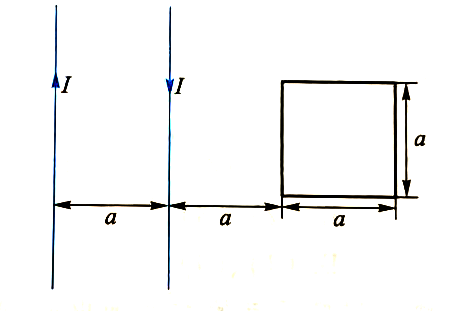
\includegraphics[width=0.33\linewidth]{figures/10-20}
		\caption{习题10-20图}
		\label{fig:10-20}
	\end{figure}
	
	\item [\textbf{10-22}] 如图~\ref{fig:10-22}~所示，在一无限长直导线附近放置一个矩形导线线框，该线框在垂直于导线方向上以匀速度$\boldsymbol{v}$向右移动，求在图示位置处线框中感应电动势的大小和方向.
	\begin{figure}[H]
		\centering
		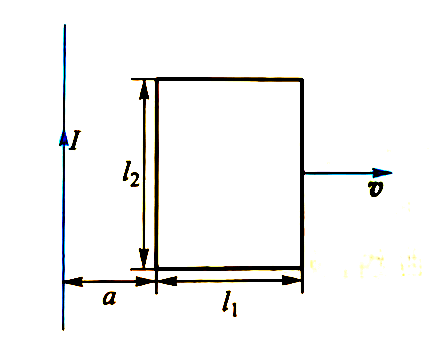
\includegraphics[width=0.3\linewidth]{figures/10-22}
		\caption{习题10-22图}
		\label{fig:10-22}
	\end{figure}
	
	\item [\textbf{10-23}] 导线ab长为l，绕过O点的垂直轴以匀角速$\boldsymbol{\omega}$转动，$aO=\boldsymbol{\frac{1}{3}l}$，磁感应强度$\boldsymbol{B}$平行于转轴，如图~\ref{fig:10-23}~所示，求：
	\begin{itemize}
		\item [(1)] ab两端的电势差;
		\item [(2)] ab两端哪端电势较高？
	\end{itemize}

	\begin{figure}[H]
		\centering
		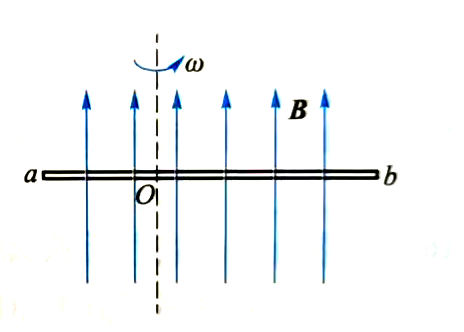
\includegraphics[width=0.4\linewidth]{figures/10-23}
		\caption{习题10-23图}
		\label{fig:10-23}
	\end{figure}
	
	\item[\textbf{L10-1}] 如图~\ref{fig:L10-1}~所示，若矩形线框静止，长直导线中的电流为
	\(I=I_{\mathrm{m}}\sin\omega t\)，求线框中产生的感应电动势.
	
	\begin{figure}[H]
		\centering
		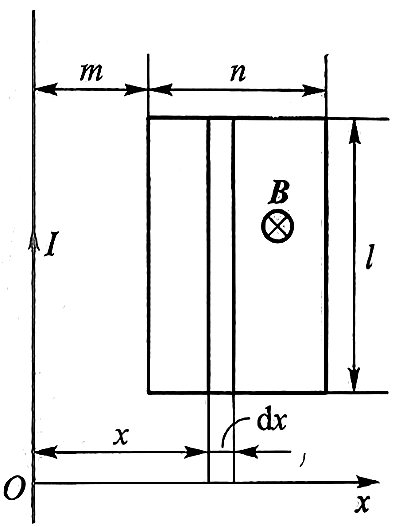
\includegraphics[width=0.25\linewidth]{figures/L10-1}
		\caption{例题10-1图}
		\label{fig:L10-1}
	\end{figure}
	
	\item[\textbf{L10-2}] 如图~\ref{fig:L10-2}~所示，在均匀磁场中，置有面积为 $S$ 的可绕 $OO'$ 轴转动的 $N$ 匝线圈.若线圈以角速度 $\omega$ 匀速转动，求线圈中的感应电动势.
	
	\begin{figure}[h]
		\centering
		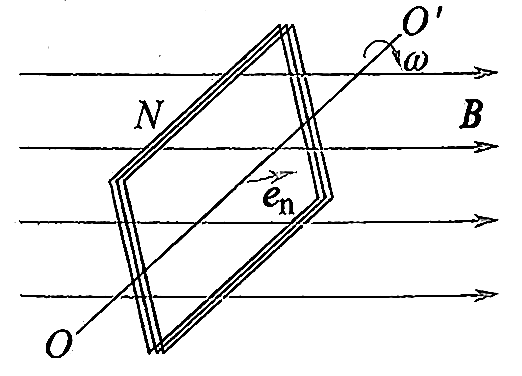
\includegraphics[width=0.3\linewidth]{figures/L10-2}
		\caption{例题10-2图}
		\label{fig:L10-2}
	\end{figure}
	
	\item[\textbf{L10-5}] 如图~\ref{fig:L10-5}~所示，在无限长直线电流 \(I\) 的磁场中，导体棒 \(ab\) 平行于电流方向以速度 \(v\) 运动，求导体棒 \(ab\) 中产生的感应电动势.
	
	\begin{figure}[H]
		\centering
		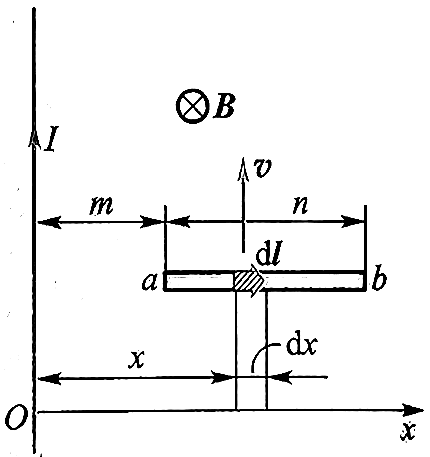
\includegraphics[width=0.3\linewidth]{figures/L10-5}
		\caption{例题10-5图}
		\label{fig:L10-5}
	\end{figure}
	
	\item[\textbf{L10-7}] 一半径为\(R\)的无限长直螺线管，其中的电流作线性变化(\(\frac{dI}{dt}=\text{常量}\))时，其内部磁场也随时间线性变化，\(\frac{dB}{dt}\)为常量，设 \(\frac{dB}{dt}\) 大小已知，求:
	
	\begin{enumerate}
		\item 管内外的感生电场 \(E_i\) 的分布.
		\item 若\(\frac{\partial B}{\partial t}=\text{常量}>0\)，\(AB\) 直导线长为 \(L\)，且距圆心 \(O\) 的垂直距离为 \(h\)，求此导线上的感应电动势.
	\end{enumerate}
	
	
\end{enumerate}


\newpage
\subsection{波动光学}

\begin{enumerate}
	\item[\textbf{11-27}] 用白光照射杨氏双缝，已知$d=1.0\,\mathrm{mm}$，$D=1.0\,\mathrm{m}$，设屏无限大.
	\begin{enumerate}
		\item 求 $\lambda=500\,\mathrm{nm}$ 的第 $4$ 级明条纹位置及明条纹间距;
		\item 求 $\lambda=600\,\mathrm{nm}$ 的光理论上在屏上可呈现的最大级数;
		\item $\lambda=500\,\mathrm{nm}$ 和 $\lambda=600\,\mathrm{nm}$ 的光在屏上什么位置开始发生重叠？
	\end{enumerate}
	
	\item[\textbf{11-30}] 在双缝干涉中，波长 $\lambda=550.0\,\mathrm{nm}$ 的单色平行光垂直入射到缝间距 $d=2\times10^{-4}\,\mathrm{m}$ 的双缝上，屏到缝间距 $D=2\,\mathrm{m}$.
	\begin{enumerate}
		\item 求中央明纹两侧的两条第 $10$ 级明条纹中心间距;
		\item 用一厚度 $e=6.6\times10^{-6}\,\mathrm{m}$、折射率 $n=1.58$ 的云母片覆盖一缝后，零级明条纹将移动到原来的第几级明条纹处？
	\end{enumerate}
	
	\item[\textbf{11-35}] 如图~\ref{fig:11-35}~所示，波长为 $680.0\,\mathrm{nm}$ 的平行光垂直照射到长为 $L=0.12\,\mathrm{m}$ 的两块玻璃片上，两玻璃片一边相互接触，另一边被直径 $d=0.048\,\mathrm{mm}$ 的细钢丝隔开.
	\begin{enumerate}
		\item 求两玻璃片间的夹角 $\theta$;
		\item 相邻两明条纹间空气薄膜的厚度差是多少？
		\item 相邻两暗条纹的间距是多少？
		\item 在玻璃片上呈现多少条明条纹？
	\end{enumerate}
	
	\begin{figure}[H]
		\centering
		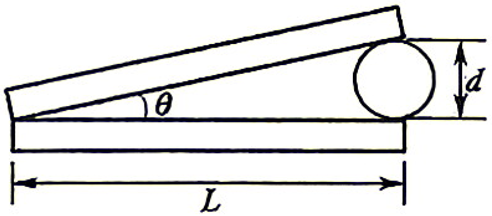
\includegraphics[width=0.3\linewidth]{figures/11-35}
		\caption{习题11-35图}
		\label{fig:11-35}
	\end{figure}
	
	
	\item[\textbf{11-43}] 波长 $\lambda=600\,\mathrm{nm}$ 的单色光垂直入射到宽度为 $a=0.01\,\mathrm{mm}$ 的单缝上，观察夫琅禾费衍射图样，透镜焦距 $f=1.0\,\mathrm{m}$，屏幕在透镜的焦平面处，求：
	\begin{enumerate}
		\item 屏上中央明条纹的宽度 $\Delta x_0$ 和半角宽度;
		\item 第二级暗纹所对应的衍射角 $\theta_2$;
		\item 第二级暗纹离透镜焦点的距离 $x_2$.
	\end{enumerate}
	
	\item[\textbf{11-44}] 波长为 $680\,\mathrm{nm}$ 的单色可见光垂直入射到缝宽为 $a=1.25\times10^{-4}\,\mathrm{cm}$ 的透射光栅上，观察到第四级谱线缺级.
	\begin{enumerate}
		\item 此光栅每厘米有多少条狭缝？
		\item 求在屏上呈现的光谱线的全部级次和条纹数.
	\end{enumerate}
	
	\item[\textbf{11-45}] 设某种波长 $\lambda_1$ 的光与波长 $\lambda_2=486.1\,\mathrm{nm}$ 的光均为平行光，它们同时垂直入射到光栅上.若 $\lambda_1$ 光的第三级光谱线与 $\lambda_2$ 光的第四级光谱线恰好重合在离中央明条纹距离为 $5\,\mathrm{mm}$ 处，设透镜焦距为 $0.50\,\mathrm{m}$.求：
	\begin{enumerate}
		\item $\lambda_1$ 的值;
		\item 光栅常量.
	\end{enumerate}
	
	\item[\textbf{11-47}] 波长为 $600\,\mathrm{nm}$ 的单色光垂直入射到一光栅上，第二和第三级明条纹分别出现在 $\sin\theta_2=0.20$ 和 $\sin\theta_3=0.30$ 处，第四级缺级，问：
	\begin{enumerate}
		\item 光栅常量是多少？
		\item 狭缝最小可能宽度有多大？
		\item 按上述选定的 $a$、$b$ 值，实际呈现的全部级次为多少？
	\end{enumerate}
	
	\item[\textbf{L11-1}] 很薄的云母片($n=1.58$)覆盖在双缝实验中的一条缝上，如图~\ref{fig:L11-1}~所示，这时屏幕上的零级明条纹移到原来的第 $7$ 级明条纹的位置上.如果入射光波长为 $550\,\mathrm{nm}$，试问此云母片的厚度为多少？
	
	\begin{figure}[H]
		\centering
		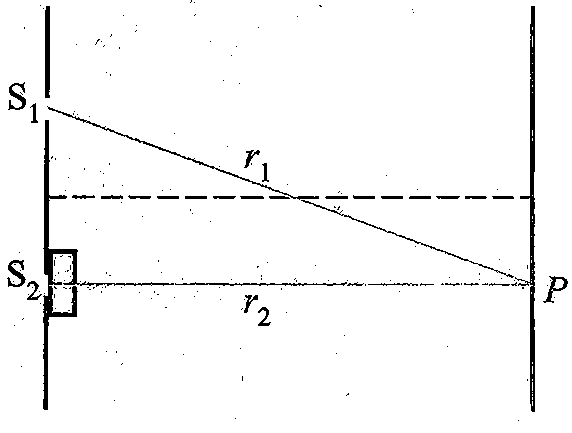
\includegraphics[width=0.25\linewidth]{figures/L11-1}
		\caption{例题11-1图}
		\label{fig:L11-1}
	\end{figure}
	
	
	\item[\textbf{L11-2}] 在一光学元件的玻璃(折射率 $n_{3}=1.5$)表面上镀一层厚度为 $e$、折射率为 $n_{2}=1.38$ 的氟化镁薄膜，为了使入射白光中对人眼最敏感的黄绿光($\lambda=550\,\mathrm{nm}$)反射最小，试求薄膜的厚度.
	
	\begin{figure}[H]
		\centering
		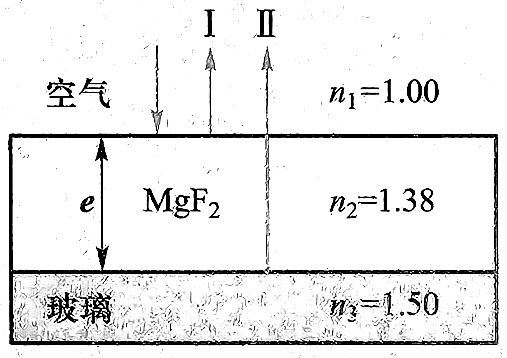
\includegraphics[width=0.3\linewidth]{figures/L11-2}
		\caption{例题11-2图}
		\label{fig:l11-2}
	\end{figure}
	
	
	\item[\textbf{L11-5}] 设光栅平面和透镜都与屏幕平行，在透射光栅上每厘米有 $5\,000$ 条刻线，用它来观察钠黄光($\lambda = 589\,\mathrm{nm}$)的光谱线.问：
	
	\begin{enumerate}
		\item 当光线垂直入射到光栅上时，能看到的光谱线的最高级数 $k_m$ 是多少？
		\item 当光线以 $\varphi = 30^\circ$ 的入射角(入射光线与光栅平面的法线的夹角)斜入射到光栅上时，能看到的光谱线的最高级数 $k'_m$ 是多少？
	\end{enumerate}
	
	
	
\end{enumerate}

\newpage